\documentclass[class=NCU_thesis, crop=false]{standalone}
\begin{document}

\chapter{實驗設計與結果}

\section{音源分離評估}
本節將比較兩個不同的音源分離模型,Aug4mss~\cite{Chiu_ChingYu2020MixingSpecific}
與本研究使用的Band-Split RNN~\cite{Luo_Yi2022MusicSourceSeparation}
在小提琴與鋼琴混合音訊資料上的表現。首先會先介紹使用的訓練資料集與測試資料集,
接著介紹模型訓練的設定、評估指標與評估結果。

\subsection{音源分離資料集}
在眾多的音訊公開資料集中,能包含多音軌錄音資料和乾淨的單音軌錄音資料可說是少之又少,
在古典樂器的音訊資料集更是如此。
在~\cite{Chiu_ChingYu2020MixingSpecific}中他們從網路上蒐集了
6小時的古典小提琴獨奏錄音與6小時的流行鋼琴獨奏錄音作為他們的訓練與驗證資料集,
但因為版權的關係,並沒有提供他們蒐集的資料集給外界使用。
因此本研究也遵循~\cite{Chiu_ChingYu2020MixingSpecific}的方式,
將小提琴與鋼琴兩種樂器的資料分開蒐集。
我們整合了多個公開資料集作為訓練資料,公開資料集包含由John Thickstun等人提供的
MusicNet~\cite{Thickstun2017Learning, Thickstun2018Invariances}、
Muneratti Ortega等人提供的Expressive Solo Violin~\cite{Muneratti_Ortega2021Expressive}與
Dong, Hao-Wen等人提供的Bach Violin Dataset~\cite{Dong_HaoWen2021Bach}。

MusicNet資料集中有330個古典音樂錄音,
錄音種類包含鋼琴獨奏、小提琴獨奏、大提琴獨奏、長笛獨奏、鋼琴與樂器合奏、管樂合奏與弦樂合奏等組合,
我們從資料集中挑選出鋼琴獨奏與小提琴獨奏的錄音資料作為訓練資料集的一部分。
Expressive Solo Violin資料集是由專業的小提琴家在同一天錄製九個不同曲子片段的錄音,
每一個片段會以不同的音樂表達方式演奏三次,並使用多個電容式麥克風同時錄音。
我們採用了資料集中所有的錄音資料(81個片段)作為訓練資料集的一部分。
Bach Violin Dataset為整合了高品質公開錄音的巴赫小提琴獨奏奏鳴曲(BWV 1001-1006)資料集,
其中包含17位小提琴家在不同的演奏場所下錄製的資料,
我們採用有提供錄音檔案的資料作為訓練資料集的一部分。

整合完畢的訓練資料集格式如\cref{table:table-ours-training-dataset}所示,
小提琴獨奏音檔的總時長為5小時24分47秒,
鋼琴獨奏音檔的總時長為5小時06分37秒,
所有資料皆為單聲道WAVE音訊格式。
\begin{table}[h]
    \centering
    \caption{整合的訓練資料集格式}
    \label{table:table-ours-training-dataset}
    \begin{tabular}{|c|c|c|}
        \hline
        \multicolumn{1}{|c|}{} & \multicolumn{1}{|c|}{小提琴音源} & \multicolumn{1}{|c|}{鋼琴音源} \\
        \hline
        總時長 & 5hr 24min 47sec & 5hr 6min 37sec \\
        \hline
        Channel & Mono & Mono \\
        \hline
        音訊格式 & WAV & WAV \\
        \hline
    \end{tabular}
\end{table}

我們根據~\cite{Chiu_ChingYu2020MixingSpecific}中切割資料集的方式,
將每種樂器的訓練資料集切成訓練集與驗證集,如\cref{table:table-ours-splited-dataset}所示。
\begin{table}[h]
    \centering
    \caption{每種樂器的訓練集與驗證集大小}
    \label{table:table-ours-splited-dataset}
    \begin{tabular}{|c|c|c|}
        \hline
        \multicolumn{1}{|c|}{} & \multicolumn{1}{|c|}{訓練集} & \multicolumn{1}{|c|}{驗證集} \\
        \hline
        小提琴 & 4hr & 1hr 24min 47sec \\
        \hline
        鋼琴 & 4hr & 1hr 6min 37sec \\
        \hline
    \end{tabular}
\end{table}

測試資料集我們採用~\cite{Chiu_ChingYu2020MixingSpecific}
所提供的公開整合測試資料集進行評估,
此資料集是從公開資料集MedleyDB~\cite{Bittner2014MedleyDB}中特別
挑選出小提琴與鋼琴的錄音所製作的測試資料集。

\colorbox{yellow}{放資料集的連結?}

\subsection{模型訓練細節} \label{training-dataset-processing}
為了公平起見,我們使用自己的公開資料集重新訓練Aug4mss模型來評估效能,
在Aug4mss的論文~\cite{Chiu_ChingYu2020MixingSpecific}中
透過控制每次迭帶的訓練樣本數設計了Data-limit與Data-rich兩種情境,
測試模型在資料缺乏與資料足夠時的表現。
因此在訓練兩種模型時,
我們參考~\cite{Chiu_ChingYu2020MixingSpecific}設定的資料筆數$N$,
$N$為在模型訓練過程中,每次迭帶從每種樂器的資料集隨機選取$N$對所混合的資料筆數。
我們針對上述兩種情況做測試。
訓練與驗證的資料筆數$N$如\cref{table:table-training-dataset-split}所示。
\begin{table}[h]
    \centering
    \caption{每次迭帶的訓練與驗證資料筆數}
    \label{table:table-training-dataset-split}
    \begin{tabular}{|c|c|c|}
        \hline
        \multicolumn{1}{|c|}{} & \multicolumn{1}{|c|}{Data-limit} & \multicolumn{1}{|c|}{Data-rich} \\
        \hline
        \textbf{訓練}資料混合筆數 & 250 pairs & 2000 pairs \\
        \hline
        \textbf{驗證}資料混合筆數 & \multicolumn{2}{|c|}{100 pairs} \\
        \hline
    \end{tabular}
\end{table}

所有訓練與測試的資料皆為44100Hz取樣率的單聲道音訊,
STFT Window size為2048,Hop size為512,並保留原始模型的設定參數。
模型訓練所使用的顯示卡為GeForce RTX™ 3080 Ti,
CPU為11th Gen Intel(R) Core(TM) i7-11700K @ 3.60GHz。

\subsection{音源分離評估指標}
我們使用~\cite{Luo_Yi2022MusicSourceSeparation}中的兩種評估指標來評估模型,
這兩種評估指標皆是基於\cref{eq:SDR-function}計算訊號失真比。
\begin{equation}
    \label{eq:SDR-function}
    SDR = 10\log _{10}
    \frac{\sum _{n}\left\lVert s(n)\right\rVert^{2} + \epsilon }
    {\sum _{n}\left\lVert s(n)-\hat{s}(n) \right\rVert^{2} + \epsilon}, s(n)\in \mathbb{R}^{2}
\end{equation}
上述公式計算同一筆資料中在離散時間$n$的訊號失真比,
$s(n)$為正確的波型,$\hat{s}(n)$為估計的波型,
另外為了避免除數為零,我們使用一個很小的常數$\epsilon = 10^{-7}$來避免這個情況。
當SDR的值越高,代表估計的波型與正確的波型越相近,分離效果越好。

下面介紹兩種評估指標的來源與計算方法:
\begin{enumerate}
    \item uSDR:Utterance-level SDR為~\cite{Yuki_Mitsufuji2021MusicDemixing}
    提出的評估方法,我們使用官方的版本針對整個訊號來計算SDR,並計算所有曲子的平均SDR數值。
    \item cSDR:Chunk-level SDR為bss\_eval指標~\cite{Vincent2006Performance}
    中計算的SDR方法,我們使用官方的版本,計算每首曲子中所有1秒區塊的SDR中位數,
    獲得每首曲子的SDR數值後再取中位數。
\end{enumerate}

% 最後將小提琴與鋼琴的SDR加總取平均

% \begin{equation}
%     \label{eq:SDR-song-function}
%     SDR_{Songs} = \frac{1}{2} (SDR_{Violin} + SDR_{Piano})
% \end{equation}

\subsection{音源分離結果比較}

根據 \ref{training-dataset-processing} 節所提到的兩種情況,
\cref{table:table-data-limit-music-source-separation}
與\cref{table:table-data-rich-music-source-separation}
為模型在Data-limit與Data-rich情況下訓練的結果。

在~\cite{Chiu_ChingYu2020MixingSpecific}
中他們加入了多種Data Augmentation方法測試模型效能,
由於本研究在訓練模型時皆採用Random mixing的方式
從訓練資料中隨機挑選每種樂器的10秒音訊進行混合,
因此本研究只比較~\cite{Chiu_ChingYu2020MixingSpecific}中Random mixing的結果。

\begin{table}[h]
    \centering
    \caption{Data-limit 結果數值比較}
    \label{table:table-data-limit-music-source-separation}
    \begin{tabular}{|c|c|c|c|}
        \hline
        \multicolumn{1}{|c|}{分離目標樂器} & \multicolumn{1}{|c|}{模型} & \multicolumn{1}{|c|}{cSDR} & \multicolumn{1}{|c|}{uSDR}\\
        \hline
        \multirow{3}*{Violin} & Aug4mss(paper) & 1.08 & No result \\
        \cline{2-4}
        ~ & Aug4mss(retrain) & 2.05 & 1.72 \\
        \cline{2-4}
        ~ & \textbf{Band-Split RNN} & \textbf{8.910} & \textbf{3.264} \\
        \hline
        \multirow{3}*{Piano} & Aug4mss(paper) & 7.43 & No result \\
        \cline{2-4}
        ~ & Aug4mss(retrain) & 11.906 & 10.974 \\
        \cline{2-4}
        ~ & \textbf{Band-Split RNN} & \textbf{14.659} & \textbf{13.460} \\
        \hline
    \end{tabular}
\end{table}

\begin{table}[h]
    \centering
    \caption{Data-rich 結果數值比較}
    \label{table:table-data-rich-music-source-separation}
    \begin{tabular}{|c|c|c|c|}
        \hline
        \multicolumn{1}{|c|}{分離目標樂器} & \multicolumn{1}{|c|}{模型} & \multicolumn{1}{|c|}{cSDR} & \multicolumn{1}{|c|}{uSDR}\\
        \hline
        \multirow{3}*{Violin} & Aug4mss(paper) & 3.84 & No result \\
        \cline{2-4}
        ~ & Aug4mss(retrain) & 5.811 & 5.666 \\
        \cline{2-4}
        ~ & \textbf{Band-Split RNN} & \textbf{11.872} & \textbf{8.297} \\
        \hline
        \multirow{3}*{Piano} & Aug4mss(paper) & 13.46 & No result \\
        \cline{2-4}
        ~ & Aug4mss(retrain) & 13.514 & 14.124 \\
        \cline{2-4}
        ~ & \textbf{Band-Split RNN} & \textbf{16.526} & \textbf{15.467} \\
        \hline
    \end{tabular}
\end{table}

在 Data-limit 的情況下,Band-Split RNN 在小提琴和鋼琴的分離效果上都是表現最為出色。
Band-Split RNN 在小提琴分離上的 cSDR 和 uSDR 分別為 9.429 和 6.767,
而在鋼琴分離上的 cSDR 和 uSDR 分別為 14.556 和 13.370。
相比之下,Aug4mss (retrain) 的結果分別為 2.05 和 1.72(小提琴),
以及 11.906 和 10.974(鋼琴)。

在 Data-rich 的情況下,Band-Split RNN 在小提琴和鋼琴的分離效果上也是表現最為出色。
Band-Split RNN 在小提琴分離上的 cSDR 和 uSDR 分別為 11.872 和 8.297,
而在鋼琴分離上的 cSDR 和 uSDR 分別為 16.526 和 15.467。
相比之下,Aug4mss (retrain) 的結果分別為 5.811 和 5.666(小提琴),
以及 13.514 和 14.124(鋼琴)。

可以注意到Aug4mss (retrain)的結果皆比Aug4mss (paper)要來的好,
可能是因為我們將原本的STFT參數改為與Band-Split RNN所設定的數值相同,
原本的Window Size從4096變為2048,Hop Size從1024改為512,因此使模型能訓練到更細部的特徵。

從\cref{table:table-data-limit-music-source-separation}與
\cref{table:table-data-rich-music-source-separation}可以看出,
不管是在資料缺少或是資料足夠的情況,Band-Split RNN皆在兩種分離目標中取得最好的數值,
我認為是因為Band-Split RNN有特別針對重要的頻帶做細部的切割,
使模型能學習到更重要的特徵。

\subsection{頻帶切割對於分離結果的影響}

在~\cite{Luo_Yi2022MusicSourceSeparation}中有針對頻帶分割對模型結果的影響做一系列的測試,
我們可以知道根據樂器不同的頻率範圍、音色特徵等等因素來調整頻帶分割的寬度,
可能會提升模型的結果。

在\ref{ch3-subst-estimate-band-split-point}節我們針對不同的樂器設計不同的頻帶切割範圍,
為了驗證此方法效果,我們針對自己設計的頻帶切割範圍,實作以下三個實驗,
\begin{enumerate}
    \item 使用~\cite{Luo_Yi2022MusicSourceSeparation}
    中效果最好的頻帶切割範圍V7訓練小提琴與鋼琴的音源分離模型
    \item 使用小提琴的頻帶切割範圍訓練鋼琴音源分離模型
    \item 使用鋼琴的頻帶切割範圍訓練小提琴音源分離模型
\end{enumerate}
為了節省訓練時間,上述實驗皆使用Data-limit的情況訓練,
我們將這些模型的結果一一列出比較,
如\cref{table:table-data-limit-mss-band-split-range-comparision}所示。

\begin{table}[h]
    \centering
    \caption{Data-limit 不同的Band-Split Bandwidth結果比較}
    \label{table:table-data-limit-mss-band-split-range-comparision}
    \begin{tabular}{|c|c|c|c|}
        \hline
        \multicolumn{1}{|c|}{分離目標樂器} & \multicolumn{1}{|c|}{Bandwidth} & \multicolumn{1}{|c|}{cSDR} & \multicolumn{1}{|c|}{uSDR}\\
        \hline
        \multirow{3}*{Violin} & Violin bandwidth version & \textbf{8.910} & \textbf{3.264} \\
        \cline{2-4}
        ~ & Piano bandwidth version & 8.796 & 3.077 \\
        \cline{2-4}
        ~ & V7 bandwidth version & 8.842 & 3.157 \\
        \hline
        \multirow{3}*{Piano} & Violin bandwidth version & 14.209 & 13.141 \\
        \cline{2-4}
        ~ & Piano bandwidth version & \textbf{14.659} & \textbf{13.460} \\
        \cline{2-4}
        ~ & V7 bandwidth version & 14.556 & 13.370 \\
        \hline
    \end{tabular}
\end{table}

當目標樂器為小提琴時,我們使用小提琴的頻帶切割範圍的訓練結果優於使用鋼琴範圍與V7範圍,
當目標樂器為鋼琴時,我們使用鋼琴的頻帶切割範圍的訓練結果優於使用小提琴範圍與V7範圍,
由此可見,當我們根據樂器的聲音特性來分配每個頻帶的細緻度,有助於音源分離的效果。
另外可以看到V7在兩種目標樂器的訓練結果表現皆為中間,且沒有與最好的效果差太多,
因此可以說V7頻帶範圍是小提琴與鋼琴都適用的範圍。

\pagebreak

\section{音樂追蹤評估}

\subsection{系統在不同速度下的追蹤結果} \label{ch4-subst-midi-tracking-results}
我們參考~\cite{Lin2020AHumanComputerDuetSystem}中的評估方法來檢測小提琴演奏追蹤系統的表現,
在~\cite{Lin2020AHumanComputerDuetSystem}中,現場演奏樂器為鋼琴,電腦輸出合奏為小提琴,
演奏曲子為貝多芬的Violin Sonata No.5, Op.24(Spring), movement I. Allegro 前25小節。
為了評估系統在不同演奏速度下的反應,他們使用四種不同速度範圍測試系統,分別為演奏正常速度(115-145bpm)、
慢速(90-120bpm)、快速(135-175bpm)、漸快(由80bpm加速至160bpm),參考音訊的速度設定為120bpm。
他們使用錄音設備錄製現場鋼琴與小提琴的演奏,
並使用節拍追蹤工具得到現場與參考鋼琴之間的節拍位置,進一步生成正確小提琴輸出位置(ground truth),
最後計算現場小提琴輸出位置與正確小提琴輸出位置的DTW對齊路徑,
使用\cref{eq:latency-function}與\cref{eq:avarage-latency-function}計算瞬間延遲與平均延遲來評估。

本研究使用的現場演奏樂器為小提琴,電腦輸出合奏為鋼琴,在演奏曲子與參考音訊的設定上我們跟隨
~\cite{Lin2020AHumanComputerDuetSystem}的設定,
然而在~\cite{Lin2020AHumanComputerDuetSystem}中並沒有提到他們是如何控制現場演奏速度的變化,
本研究為了能客觀地控制速度變化並計算評估結果,
我們將現場演奏的部分改為使用隨機生成速度的MIDI檔案來評估,
由於MIDI檔案擁有音符開始時間、節拍等等資訊,因此能精準地計算延遲,此外,
我們可以透過現場MIDI檔案生成正確的鋼琴輸出音訊,因此不需要額外的節拍追蹤工具輔助。
雖然現場演奏為預先設定好的檔案,但這並不影響即時的效果,現場音訊還是會以串流的方式進行處理。

\cref{fig:different-speed-midi-score-5bars}為在四種不同速度範圍下隨機生成的MIDI檔案,
我們透過讀取MIDI檔案中每個MIDI事件,將每個MIDI事件設定為有50\%的機率可以在速度範圍下隨機設定速度。
\cref{fig:slow-midi-5bars}為在慢速(90-120bpm)範圍的MIDI檔案、
\cref{fig:normal-midi-5bars}為在正常速度(115-145bpm)範圍的MIDI檔案、
\cref{fig:fast-midi-5bars}為在快速(135-175bpm)範圍的MIDI檔案,
可以看到每個有設定速度的MIDI事件,其速度設定都在對應的範圍中。
另外\cref{fig:accelerate-midi-5bars}為漸快(由80bpm加速至160bpm)範圍的MIDI檔案,
我們平均的將速度範圍分配到每個MIDI事件上,模擬漸快的情況。

\begin{figure}[H]
    %\captionsetup[subfigure]{labelformat=empty} % 完全隱藏圖號
    \centering
    \subcaptionbox
    {慢(90-120bpm)
    \label{fig:slow-midi-5bars}}
    {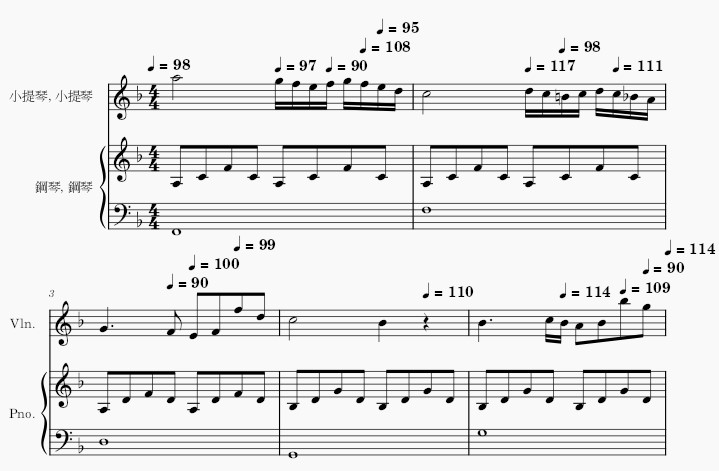
\includegraphics[width=0.4\linewidth, height=0.4\linewidth]{ch4/fig-midi-slow-score.jpg}}
    ~
    \subcaptionbox
    {一般(115-145bpm)
    \label{fig:normal-midi-5bars}}
    {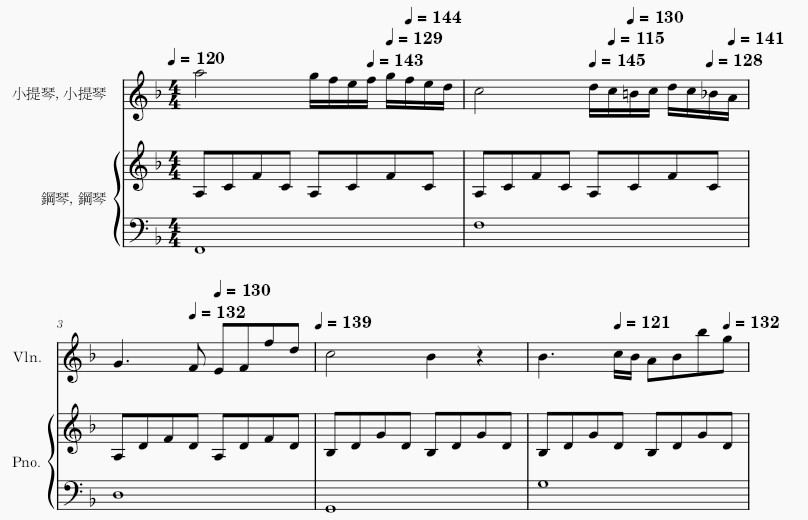
\includegraphics[width=0.4\linewidth, height=0.4\linewidth]{ch4/fig-midi-normal-score.jpg}}
    ~
    \subcaptionbox
    {快(135-175bpm)
    \label{fig:fast-midi-5bars}}
    {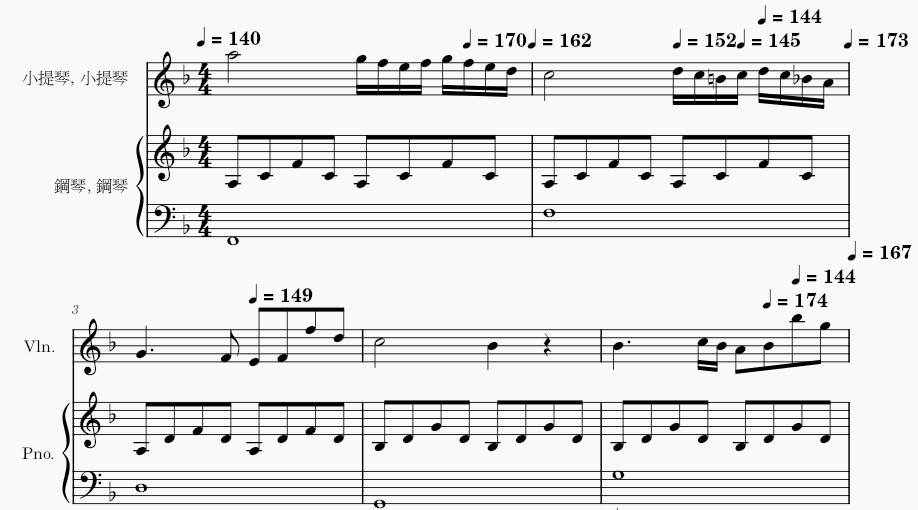
\includegraphics[width=0.4\linewidth, height=0.4\linewidth]{ch4/fig-midi-fast-score.jpg}}
    ~
    \subcaptionbox
    {加速(80$ \rightarrow $160bpm)
    \label{fig:accelerate-midi-5bars}}
    {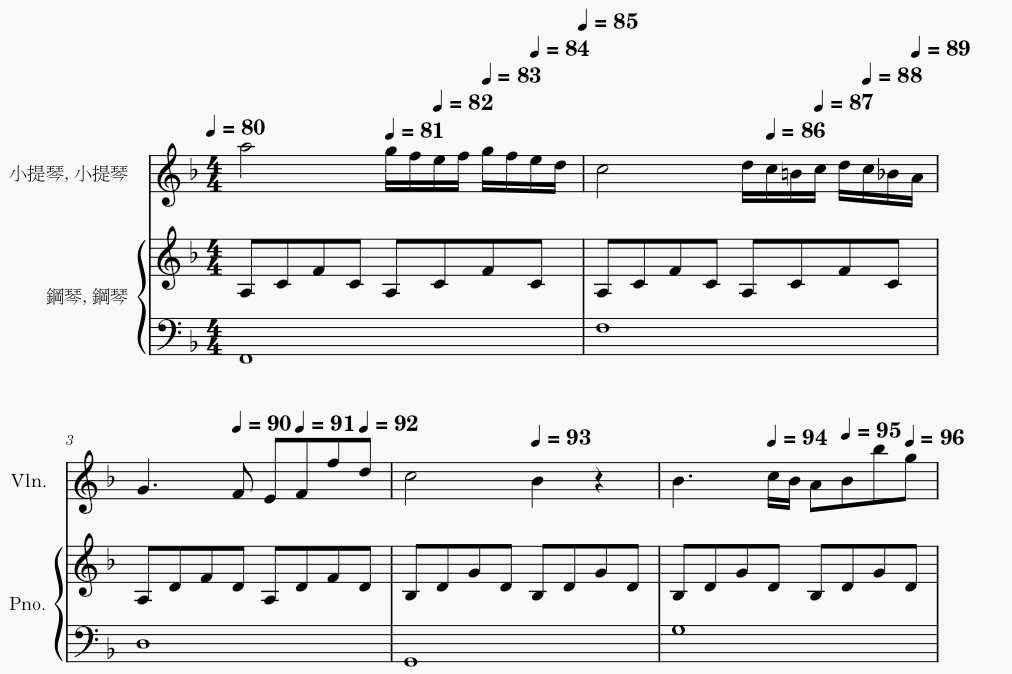
\includegraphics[width=0.4\linewidth, height=0.4\linewidth]{ch4/fig-midi-accelerate-score.jpg}}
    \caption{四種不同速度範圍的MIDI樂譜前五小節}
    \label{fig:different-speed-midi-score-5bars}
\end{figure}

由於正確的鋼琴輸出音訊已經透過MIDI檔案生成,
% 因此我們只需要使用追蹤結果與正確的鋼琴輸出音訊計算DTW對齊路徑,
因此我們只需要將正確伴奏音訊$Acc_{gt}$與追蹤系統估計的伴奏音訊$Acc_{out}$計算DTW對齊路徑,
由於伴奏音訊的時間長度是一致的,
因此可以根據\cref{eq:latency-function}
算出$Acc_{out}$在$Acc_{gt}$上的瞬間延遲(latency)。
\begin{equation}
    \label{eq:latency-function}
    \Delta [t_i] := t_j - t_i
\end{equation}

$t_i$為$Acc_{out}$的時間點,$t_j$為$Acc_{gt}$的時間點,
當$t_i = t_j$時,代表在這個時間點兩段音訊是對齊的,
當$t_i > t_j$時,代表$Acc_{out}$比$Acc_{gt}$還要快,
當$t_i < t_j$時,代表$Acc_{out}$比$Acc_{gt}$還要慢。

我們也用\cref{eq:avarage-latency-function}衡量整首曲子的平均延遲,
計算方式為將每個時間點的瞬間延遲取絕對值後加總,並除以曲子的長度$T$。
$| \Delta t\vert $為現場伴奏音訊的延遲。
\begin{equation}
    \label{eq:avarage-latency-function}
    \frac{1}{T} \sum _{t=0}^{T} | \Delta [t] \vert 
\end{equation}

\cref{fig:fig-ch4-slow-and-normal-latency-results}與\cref{fig:fig-ch4-fast-and-accelerate-latency-results}
顯示系統在四種速度變化下隨時間變化的延遲圖,也就是現場系統伴奏比正確伴奏要提前或落後多少個16分音符。
藍色線為系統延遲的16分音符數量,橘色線為當下的速度(bpm)。
\cref{fig:fig-slow-latency}是慢速時系統隨時間變化的延遲,可以看到系統在一開始雖然動盪較大,
但都保持在不超過2個16分音符的延遲下穩定追蹤,即使節拍動盪很大也不影響到系統的穩定性,
最後的平均延遲為55.04ms。
\cref{fig:fig-fast-latency}是快速時系統隨時間變化的延遲,
與慢速的延遲圖很像,但動盪較大,這可能是因為快速的速度範圍與參考的速度相差較多,
因此導致系統在追蹤時較容易有延遲,最後的平均延遲為62.96ms。
\cref{fig:fig-accelerate-latency}是漸快時系統隨時間變化的延遲,
由於一開始速度較慢,因此導致系統剛開始追蹤時動盪較大,當速度慢慢回升到接近參考音訊的速度時,
可以看到動盪越來越小,最後的平均延遲為58.23ms。
另外可以發現在第五小節(m5)與第七小節(m7)時,四種速度的延遲皆為正延遲,也就是比起正確的時間點還要提前,
可能是因為剛好那個時間點為休止符,也就是沒有音樂,因此造成系統先對齊到了最後面的靜音時間點並等待,
導致延遲。

\begin{figure}[H]
    %\captionsetup[subfigure]{labelformat=empty} % 完全隱藏圖號
    \centering
    \subcaptionbox
    {慢(90-120bpm) 平均延遲:55.04毫秒
    \label{fig:fig-slow-latency}}
    {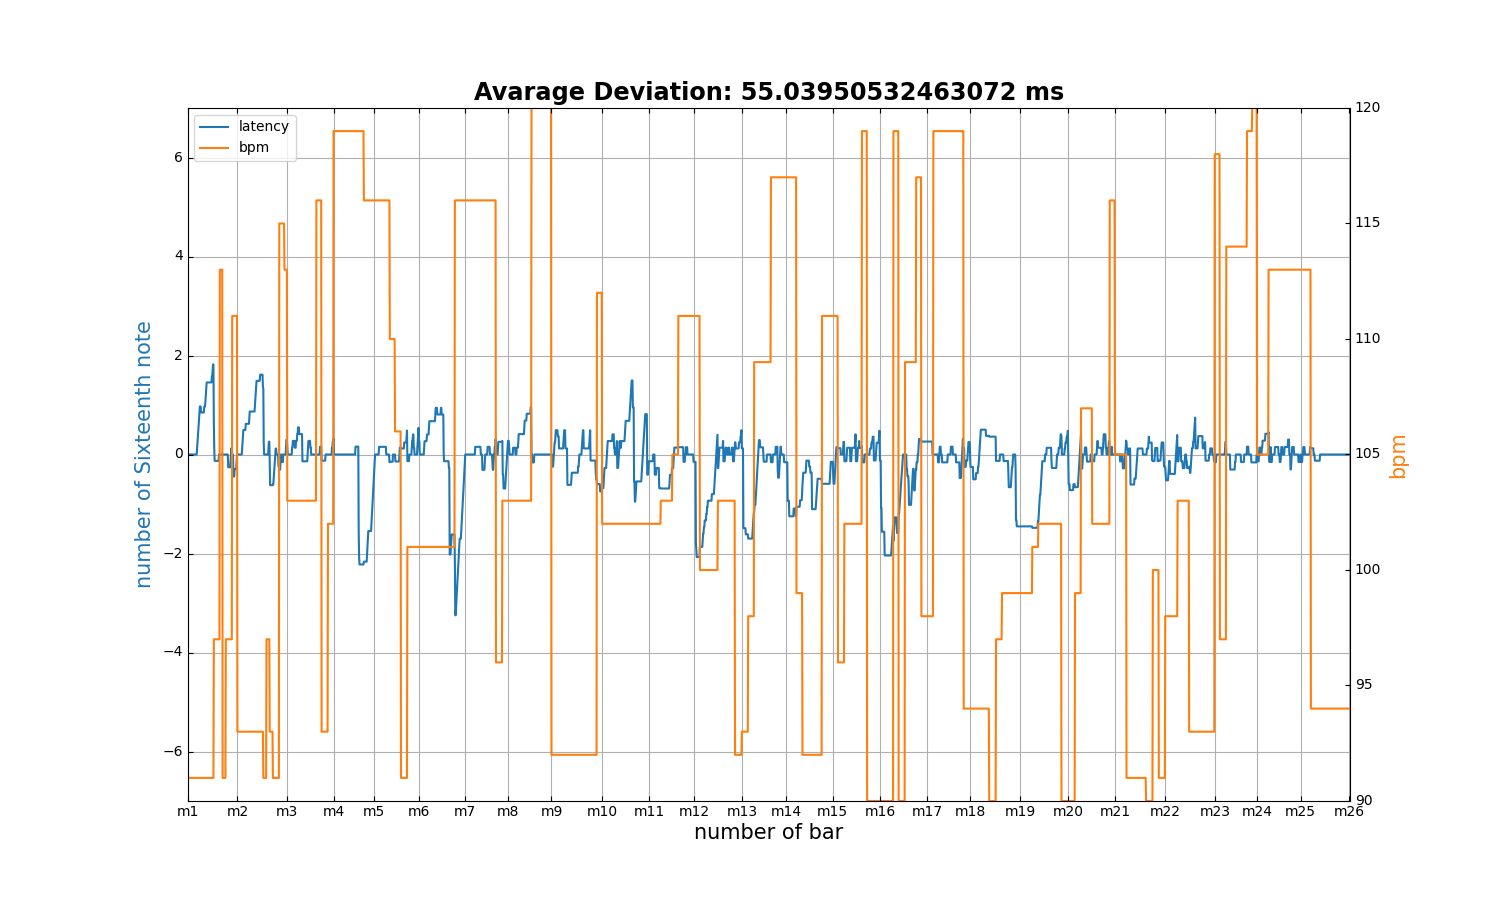
\includegraphics[width=\linewidth]{ch4/fig-slow-latency.png}}
    ~
    \subcaptionbox
    {一般(115-145bpm) 平均延遲:35.81毫秒
    \label{fig:fig-normal-latency}}
    {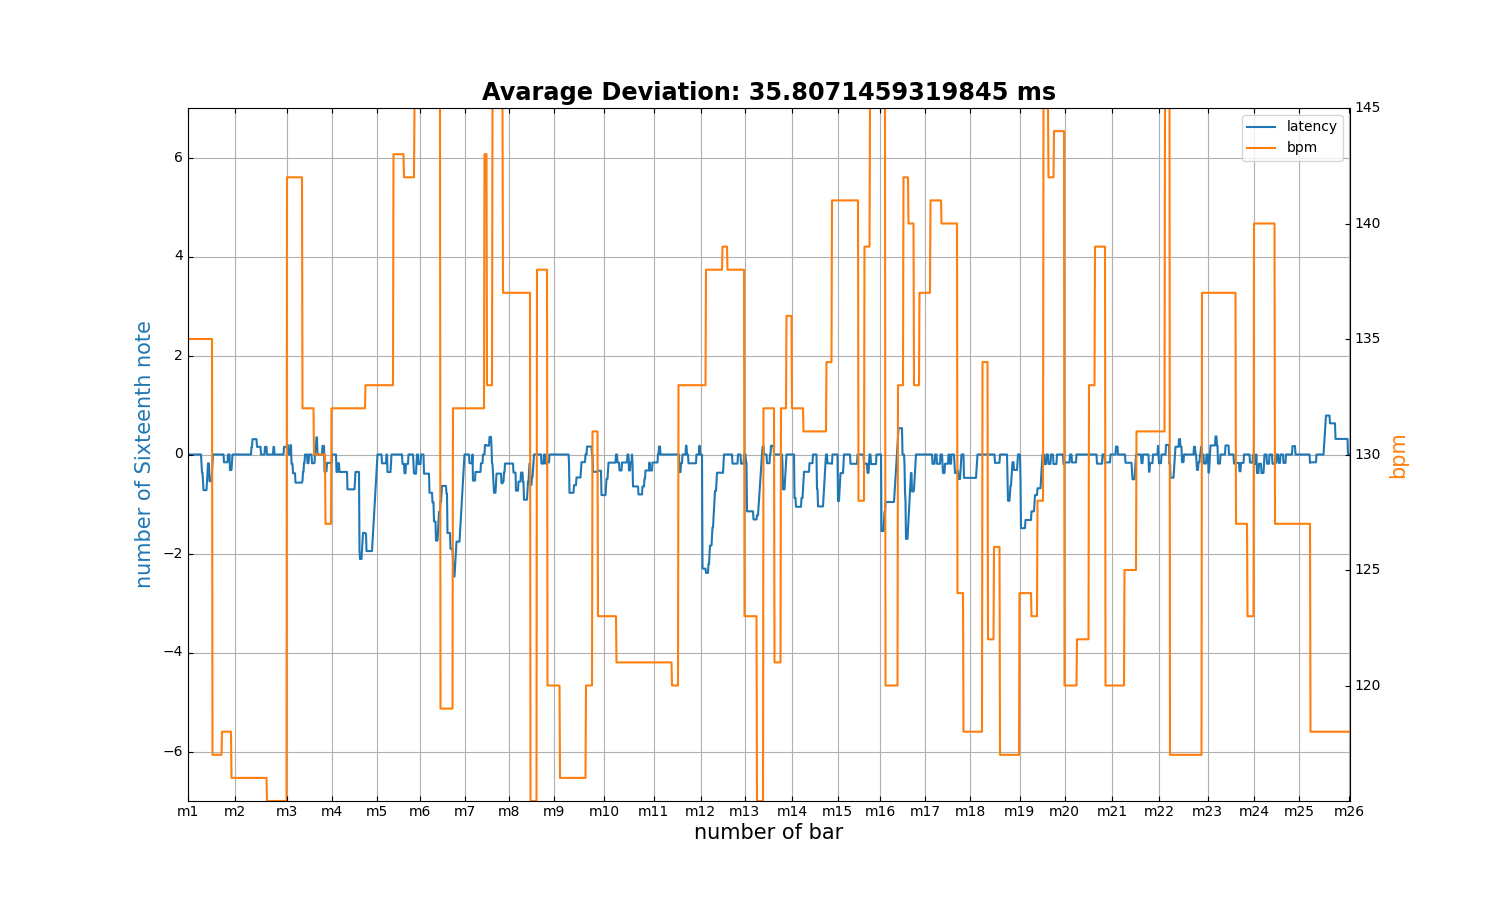
\includegraphics[width=\linewidth]{ch4/fig-normal-latency.png}}
    \caption{系統在慢、一般速度的延遲時間}
    \label{fig:fig-ch4-slow-and-normal-latency-results}
\end{figure}

\begin{figure}[H]
    %\captionsetup[subfigure]{labelformat=empty} % 完全隱藏圖號
    \centering
    \subcaptionbox
    {快(135-175bpm) 平均延遲:62.96毫秒
    \label{fig:fig-fast-latency}}
    {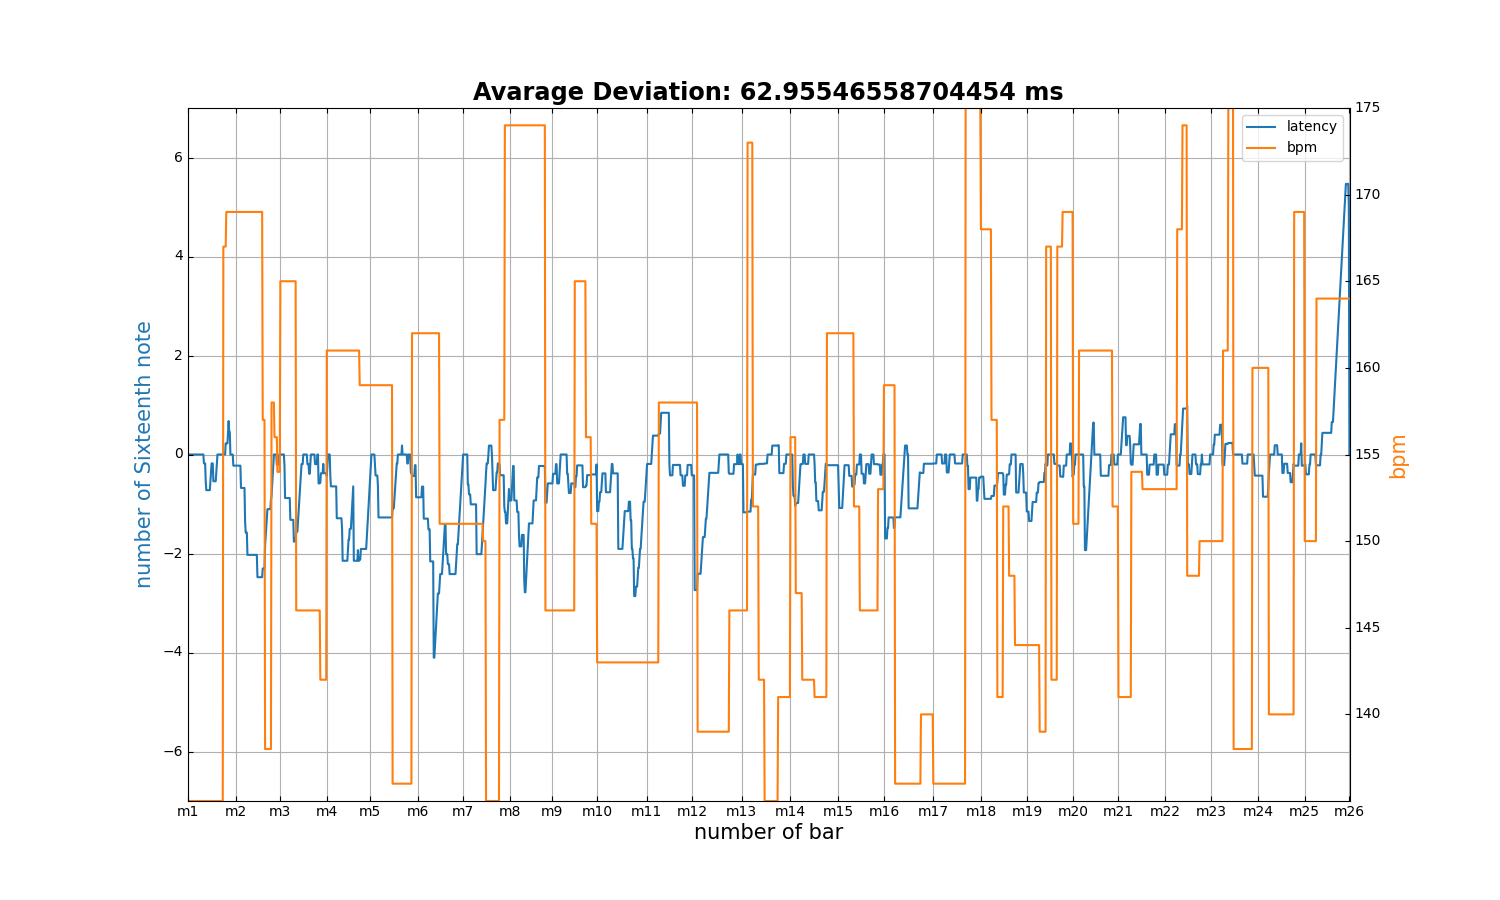
\includegraphics[width=\linewidth]{ch4/fig-fast-latency.png}}
    ~
    \subcaptionbox
    {加速(80$ \rightarrow $160bpm) 平均延遲:58.73毫秒
    \label{fig:fig-accelerate-latency}}
    {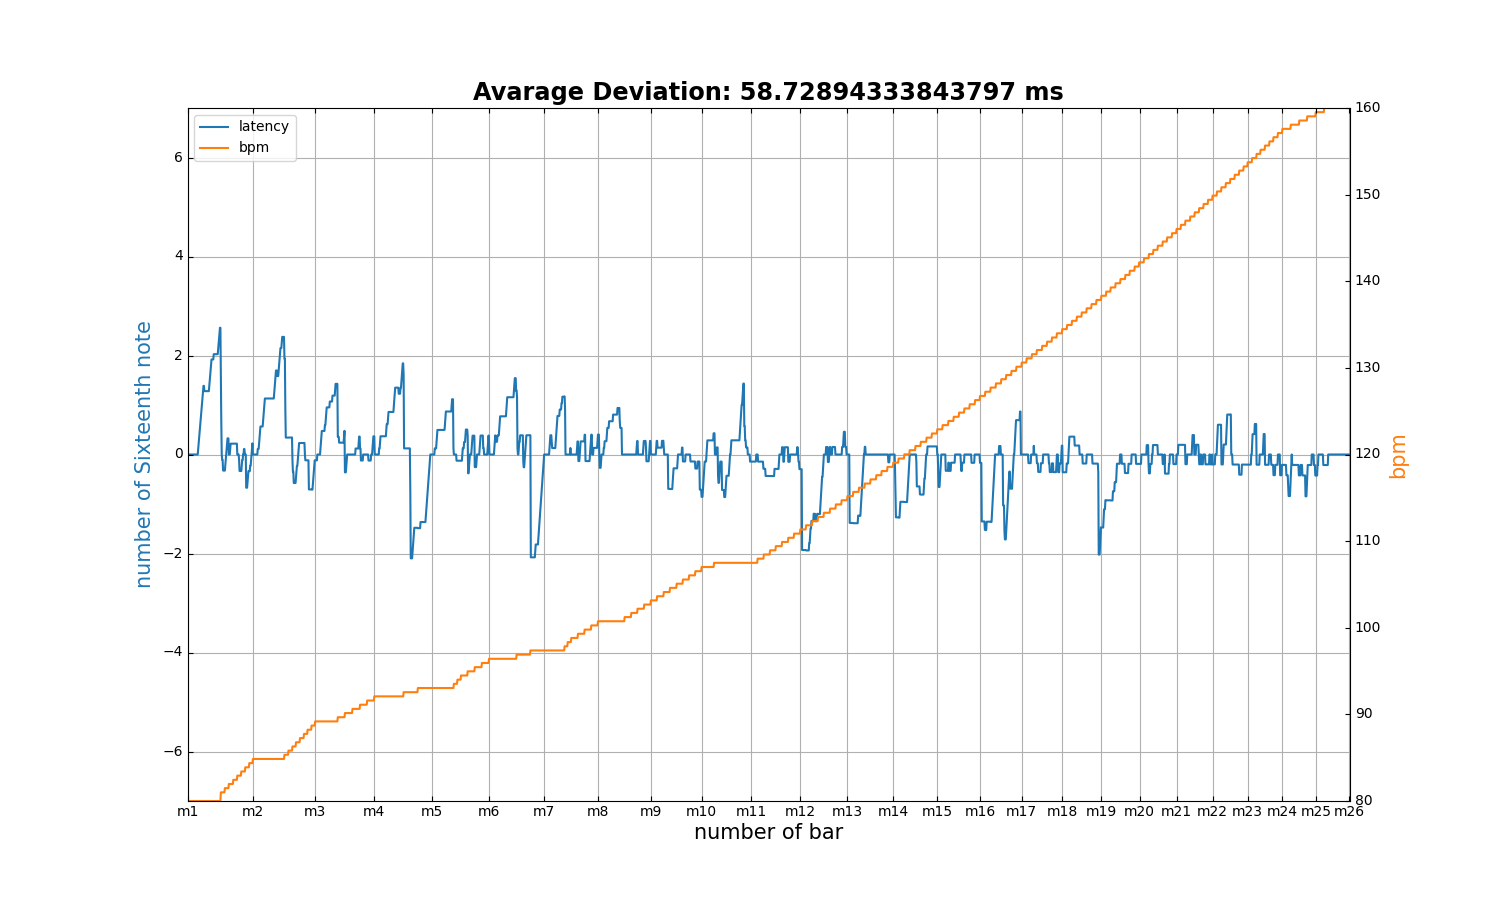
\includegraphics[width=\linewidth]{ch4/fig-accelerate-latency.png}}
    \caption{系統在快、加速速度的延遲時間}
    \label{fig:fig-ch4-fast-and-accelerate-latency-results}
\end{figure}


另外我們也顯示了四種速度的對齊路徑結果圖,橫軸為現場音訊的時間點,縱軸為參考音訊的時間點,
熱點圖的顏色代表在時間點$(i, j)$的累積距離成本值,成本值越高顏色越接近黃色。
(a)圖為追蹤系統在執行時所輸出的結果圖,
(b)圖為離線對齊路徑與線上對齊路徑的比較圖,離線對齊路徑使用DTW計算。

\cref{fig:fig-ch4-slow-tracking-results}在大部分的時間點,速度會比參考音訊的速度要慢,
因此可以看到\cref{fig:slow-tracking-output}在某些區間(例如live約600frames時)
綠色的點所連成的線較為平緩,代表此區間系統輸出較多相同的參考音訊時間點來等待現場音訊。
在\cref{fig:slow-comparision-output}的表現上,幾乎與離線對齊時的最佳路徑是一致的。
% 只是可能系統上一些無法避免的延遲(例如接收串流音訊),造成兩條路徑並不是完整的重合。

\begin{figure}[H]
    %\captionsetup[subfigure]{labelformat=empty} % 完全隱藏圖號
    \centering
    \subcaptionbox
    {
    \label{fig:slow-tracking-output}}
    {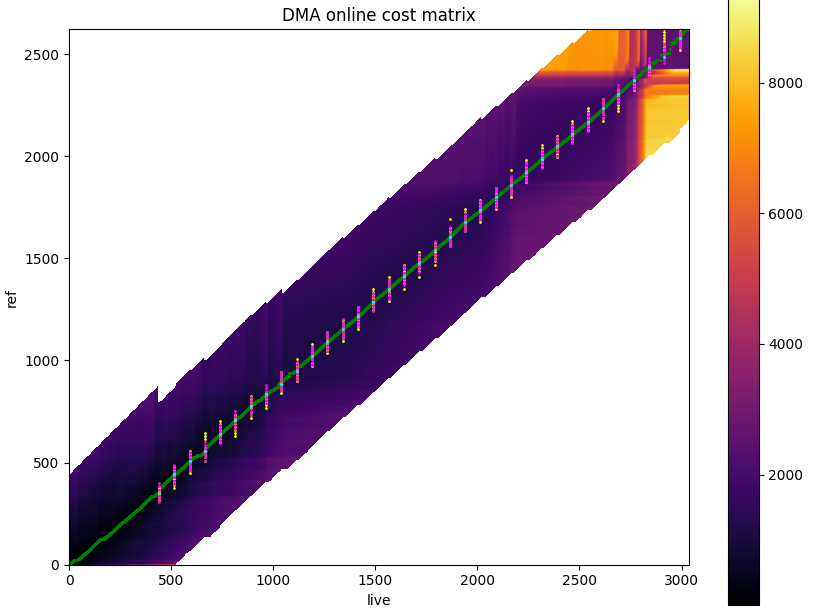
\includegraphics[scale=0.36]{ch4/fig-slow-tracking-system-output.png}}
    ~
    \subcaptionbox
    {
    \label{fig:slow-comparision-output}}
    {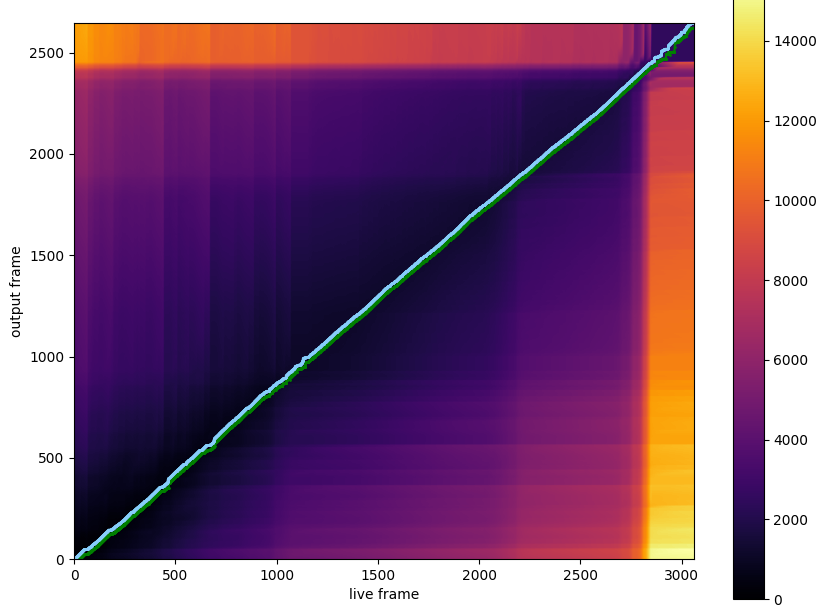
\includegraphics[scale=0.36]{ch4/fig-slow-offline-and-online-output.png}}
    \caption{慢(90-120bpm)}
    \label{fig:fig-ch4-slow-tracking-results}
\end{figure}

\cref{fig:fig-ch4-normal-tracking-results}的速度與參考音訊是最接近的,
因此在\cref{fig:normal-tracking-output}幾乎不會有波動,\cref{{fig:normal-comparision-output}}
也是表現得與離線對齊路徑相當。

\begin{figure}[H]
    %\captionsetup[subfigure]{labelformat=empty} % 完全隱藏圖號
    \centering
    \subcaptionbox
    {
    \label{fig:normal-tracking-output}}
    {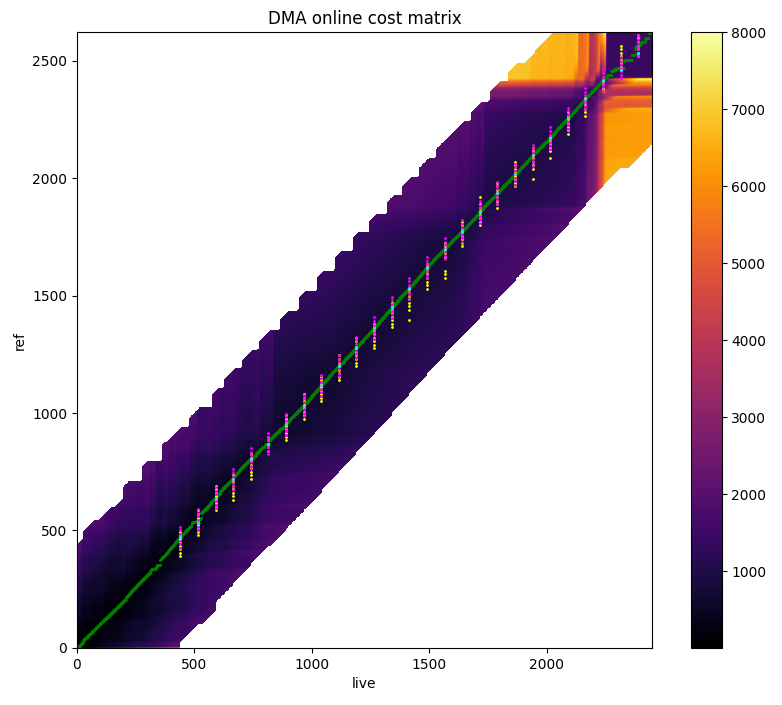
\includegraphics[scale=0.36]{ch4/fig-normal-tracking-system-output.png}}
    ~
    \subcaptionbox
    {
    \label{fig:normal-comparision-output}}
    {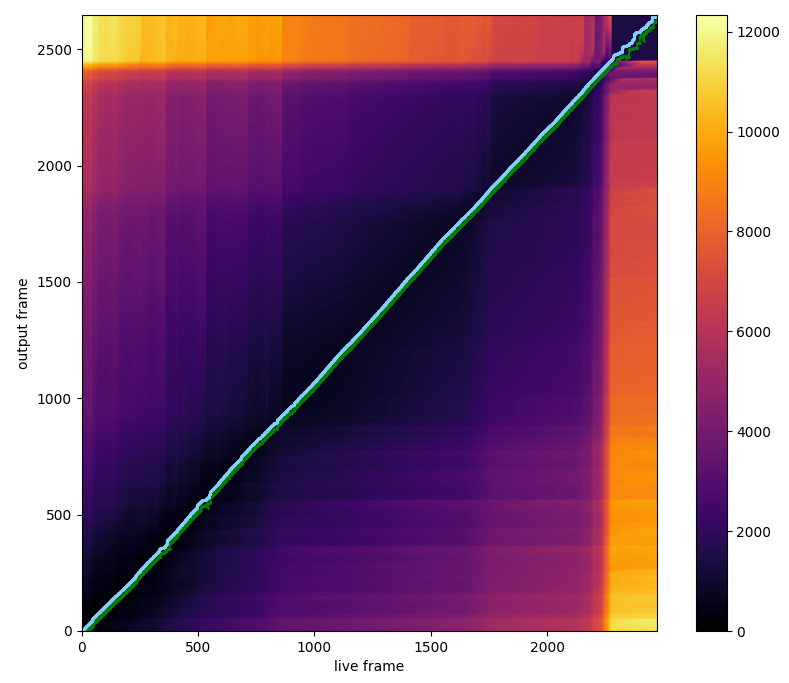
\includegraphics[scale=0.36]{ch4/fig-normal-offline-and-online-output.png}}
    \caption{一般(115-145bpm)}
    \label{fig:fig-ch4-normal-tracking-results}
\end{figure}

\cref{fig:fig-ch4-fast-tracking-results}在大部分的時間點,速度會比參考音訊的速度要快,
因此可以看到\cref{fig:fast-tracking-output}在某些區間(例如live約450frames時)
輸出路徑會呈現斷斷續續的點,代表此區間系統在輸出時認為目前現場音訊的時間點必須對齊到更後面的參考音訊,
在\cref{fig:fast-comparision-output}的表現上,雖然參考音訊的時間點並不是連續的,
但可以看到整體路徑與離線對齊路徑還是一致的。

\begin{figure}[H]
    %\captionsetup[subfigure]{labelformat=empty} % 完全隱藏圖號
    \centering
    \subcaptionbox
    {
    \label{fig:fast-tracking-output}}
    {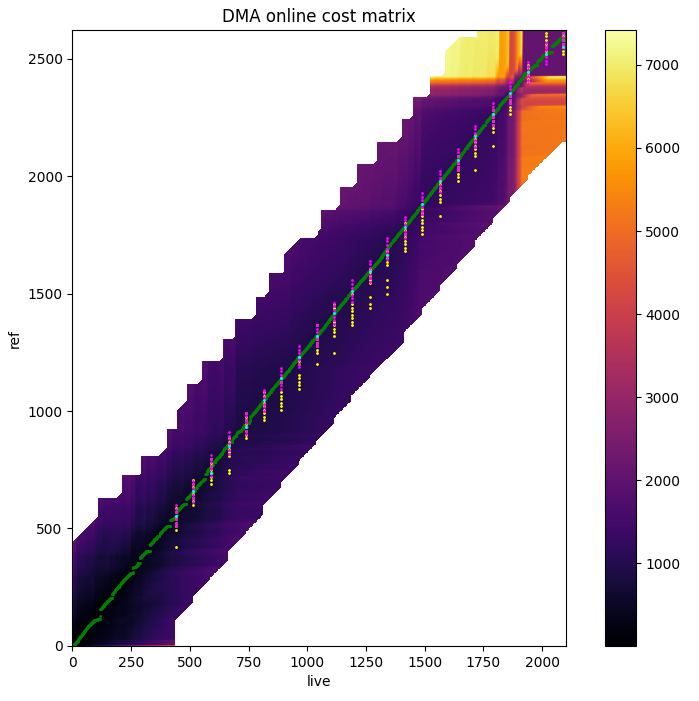
\includegraphics[scale=0.36]{ch4/fig-fast-tracking-system-output.png}}
    ~
    \subcaptionbox
    {
    \label{fig:fast-comparision-output}}
    {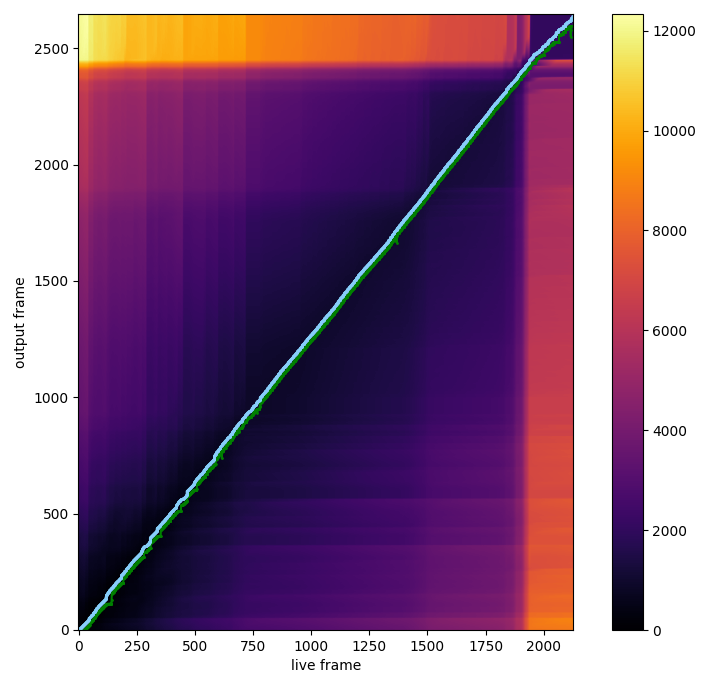
\includegraphics[scale=0.36]{ch4/fig-fast-offline-and-online-output.png}}
    \caption{快(135-175bpm)}
    \label{fig:fig-ch4-fast-tracking-results}
\end{figure}

\cref{fig:fig-ch4-accelerate-tracking-results}涵蓋了整個慢到快的速度區間,
可以看到\cref{fig:accelerate-tracking-output}在前面速度較慢時輸出相同的點的狀況較多,
當現場音訊演奏越來越快,輸出點所連成的線的斜率越來越高。
在\cref{fig:accelerate-comparision-output}的表現上,與離線對齊路徑也是呈現一致。

\begin{figure}[H]
    %\captionsetup[subfigure]{labelformat=empty} % 完全隱藏圖號
    \centering
    \subcaptionbox
    {
    \label{fig:accelerate-tracking-output}}
    {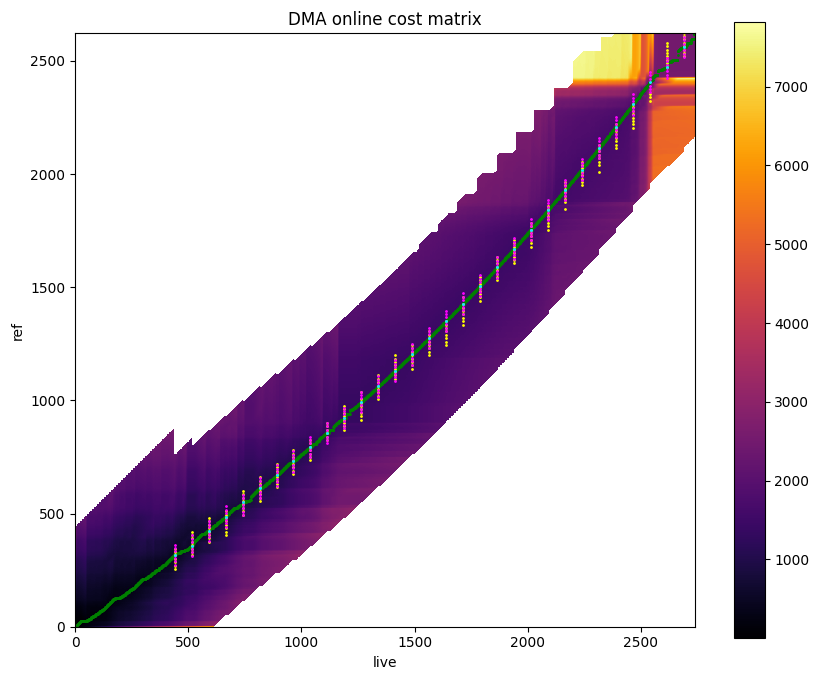
\includegraphics[scale=0.36]{ch4/fig-accelerate-tracking-system-output.png}}
    ~
    \subcaptionbox
    {
    \label{fig:accelerate-comparision-output}}
    {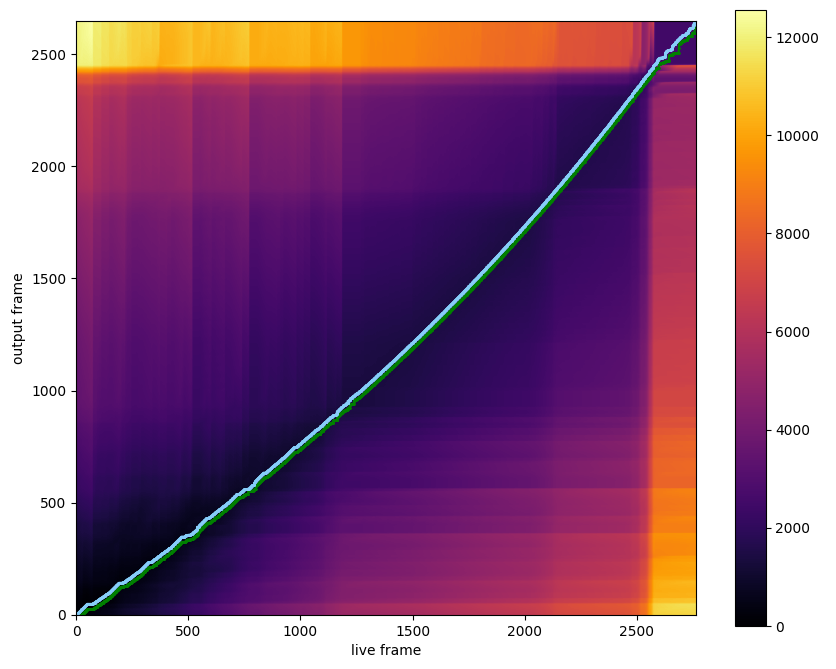
\includegraphics[scale=0.36]{ch4/fig-accelerate-offline-and-online-output.png}}
    \caption{加速(80$ \rightarrow $160bpm)}
    \label{fig:fig-ch4-accelerate-tracking-results}
\end{figure}

上述結果的音訊檔案可從{\colorbox{yellow}{github}}聆聽。

% cost matrix對齊圖
% 放MIDI隨機生成速度的那些評估圖

\subsection{系統在使用音源分離音訊做為參考特徵的追蹤結果}
為了評估系統是否在不同特徵下也能有好的追蹤結果,
我們使用與\ref{ch4-subst-midi-tracking-results}節相同的曲子,
在網路上找到由kopikostar演奏的小提琴與鋼琴合奏版本\cite{kopikostar2024Beethoven},
並對此混合音訊做音源分離,將分離結果作為參考音訊與伴奏音訊。
分離結果的音檔可至此連結聆聽{\colorbox{yellow}{github}}。

我們實際演奏現場音訊,並演奏了四種不同速度,分別為110bpm、120bpm、130bpm與140bpm,
此四種速度為這首曲子最常出現的演奏速度。
演奏時,為了保持演奏速度的平穩,我們皆使用節拍器來輔助,
我們也演奏了自由速度版本,也就是不使用節拍器,與鋼琴互相配合演奏。
在演奏時使用AKG C519 M 電容式麥克風收錄音訊,監聽耳機為Sony MDR 7506,
並使用Focusrite Scarlett 2i2錄音介面處理類比與數位訊號。

由於沒有正確的伴奏音訊(Ground truth),因此我們無法使用\ref{ch4-subst-midi-tracking-results}節的方法來評估效果。
我們改由計算系統輸出路徑與DTW離線對齊路徑的平均延遲幀數來評估系統在線上追蹤的表現,
這邊的平均延遲幀數代表的是對於線上追蹤表現,是否提前或落後離線追蹤表現。

下圖為五種不同速度的對齊路徑結果圖,橫軸為現場音訊的時間點,縱軸為參考音訊的時間點,
(a)圖為追蹤系統在執行時所輸出的結果圖,
(b)圖為離線對齊路徑與線上對齊路徑的比較圖與平均延遲幀數。

\cref{fig:fig-ch4-mss-110bpm-tracking-results}為速度110bpm下的追蹤結果,
由\cref{fig:mss-110bpm-tracking-output}的xy軸可以看出現場音訊的速度比參考音訊要來的慢,
因此會出現等待的情況,例如live frame=700的時候。
\cref{fig:mss-110bpm-comparision-output}顯示了追蹤結果與離線計算結果的延遲為26.62幀,
約為532ms左右。

\begin{figure}[H]
    %\captionsetup[subfigure]{labelformat=empty} % 完全隱藏圖號
    \centering
    \subcaptionbox
    {
    \label{fig:mss-110bpm-tracking-output}}
    {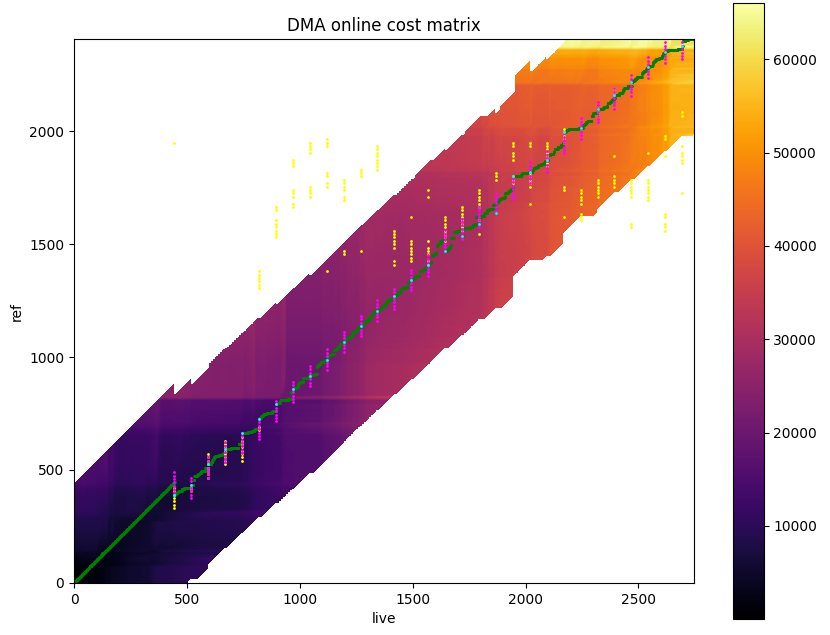
\includegraphics[scale=0.36]{ch4/fig-mss-110bpm-tracking-system-output.png}}
    ~
    \subcaptionbox
    {
    \label{fig:mss-110bpm-comparision-output}}
    {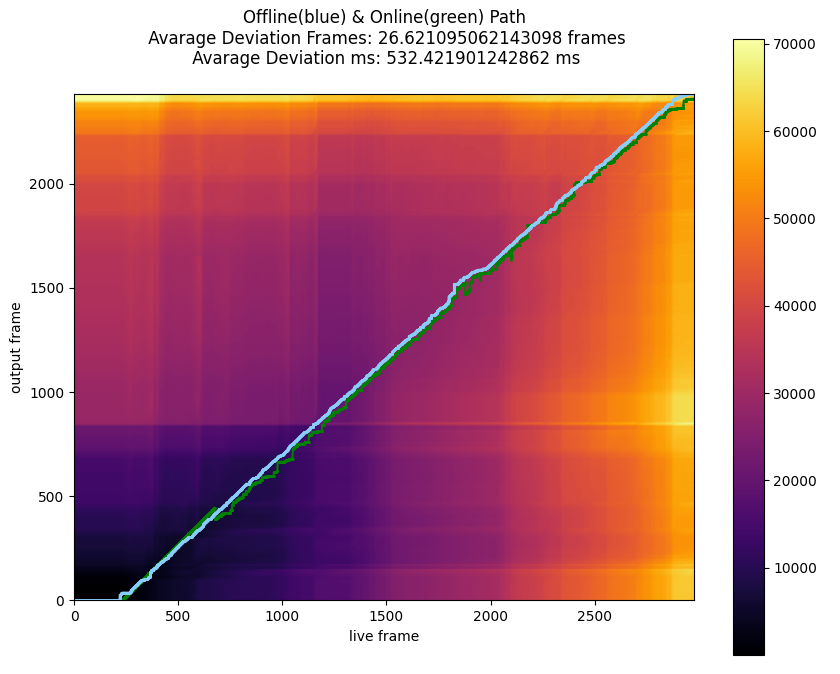
\includegraphics[scale=0.36]{ch4/fig-mss-110bpm-offline-and-online-output.png}}
    \caption{110bpm 平均延遲:26.62 幀}
    \label{fig:fig-ch4-mss-110bpm-tracking-results}
\end{figure}

\cref{fig:fig-ch4-mss-120bpm-tracking-results}為速度120bpm下的追蹤結果,
由\cref{fig:mss-120bpm-tracking-output}的xy軸可以看出現場音訊的速度也是比參考音訊的速度稍慢,
\cref{fig:mss-120bpm-comparision-output}顯示了追蹤結果與離線計算結果的延遲為27.98幀,
約為560ms左右。

\begin{figure}[H]
    %\captionsetup[subfigure]{labelformat=empty} % 完全隱藏圖號
    \centering
    \subcaptionbox
    {
    \label{fig:mss-120bpm-tracking-output}}
    {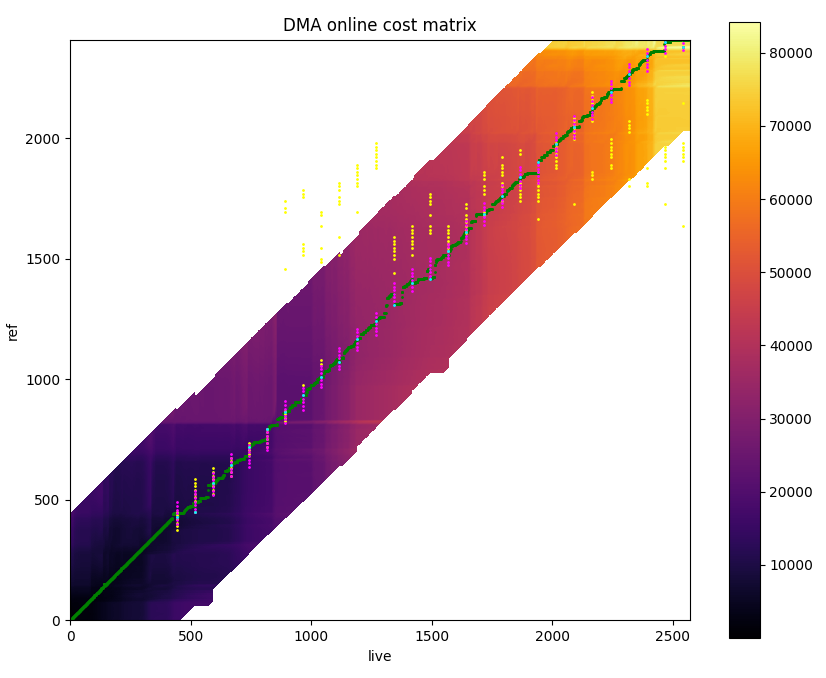
\includegraphics[scale=0.36]{ch4/fig-mss-120bpm-tracking-system-output.png}}
    ~
    \subcaptionbox
    {
    \label{fig:mss-120bpm-comparision-output}}
    {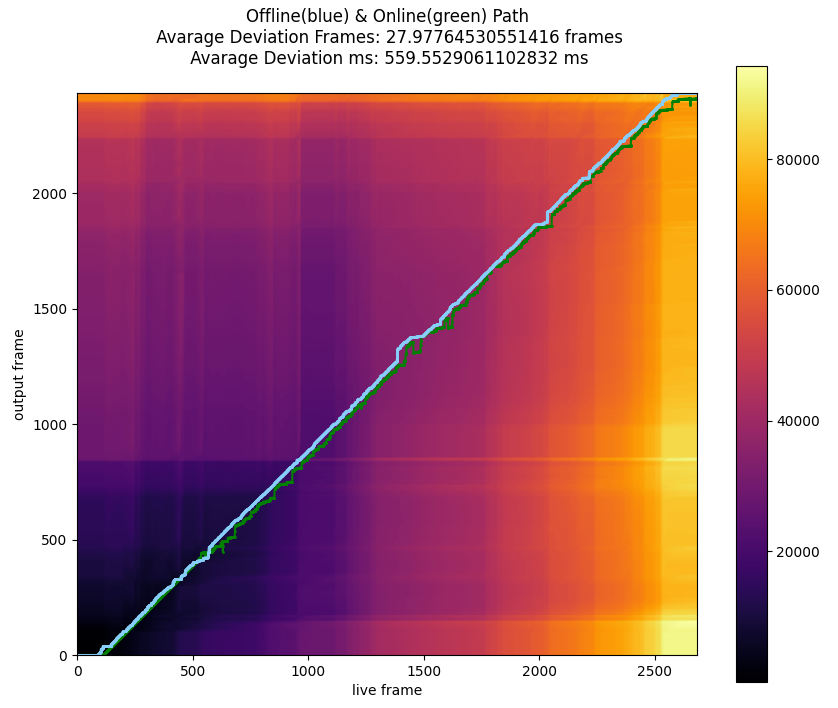
\includegraphics[scale=0.36]{ch4/fig-mss-120bpm-offline-and-online-output.png}}
    \caption{120bpm 平均延遲:27.98 幀}
    \label{fig:fig-ch4-mss-120bpm-tracking-results}
\end{figure}

\cref{fig:fig-ch4-mss-130bpm-tracking-results}為速度130bpm下的追蹤結果,
由\cref{fig:mss-130bpm-tracking-output}的xy軸可以看出現場音訊與參考音訊的速度較為相近,
但可能因為特徵差距的關係使追蹤結果並沒有比起前面的結果要好。
\cref{fig:mss-130bpm-comparision-output}顯示了追蹤結果與離線計算結果的延遲為37.49幀,
約為750ms左右。

\begin{figure}[H]
    %\captionsetup[subfigure]{labelformat=empty} % 完全隱藏圖號
    \centering
    \subcaptionbox
    {
    \label{fig:mss-130bpm-tracking-output}}
    {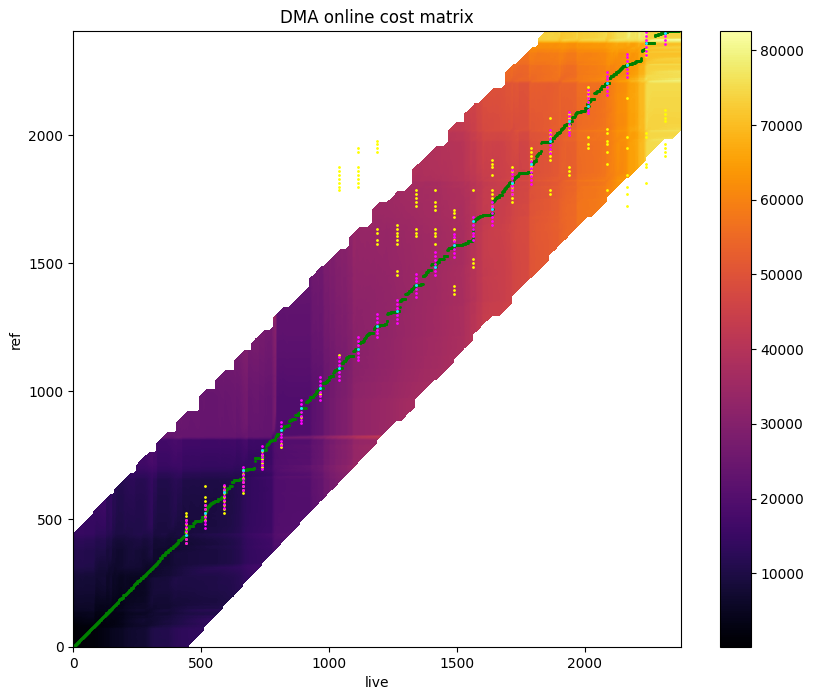
\includegraphics[scale=0.36]{ch4/fig-mss-130bpm-tracking-system-output.png}}
    ~
    \subcaptionbox
    {
    \label{fig:mss-130bpm-comparision-output}}
    {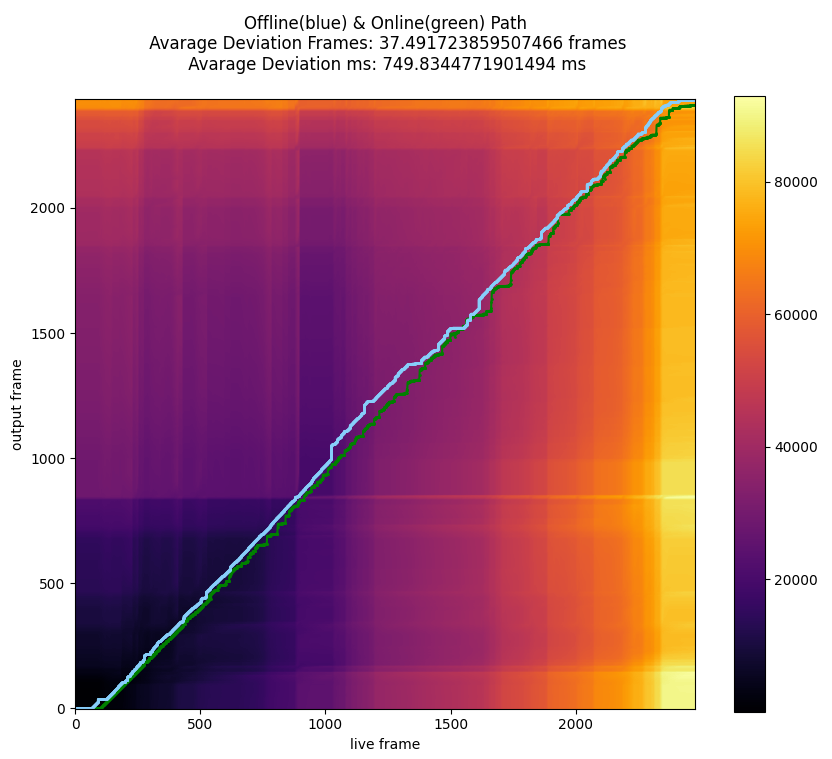
\includegraphics[scale=0.36]{ch4/fig-mss-130bpm-offline-and-online-output.png}}
    \caption{130bpm 平均延遲:37.49 幀}
    \label{fig:fig-ch4-mss-130bpm-tracking-results}
\end{figure}

\cref{fig:fig-ch4-mss-140bpm-tracking-results}為速度140bpm下的追蹤結果,
由\cref{fig:mss-140bpm-tracking-output}的xy軸可以看出現場音訊比參考音訊的速度稍快一些,
在live frame約500的時候,可以看到追蹤的路徑並不穩定,此時靠著RPE的粗略估計位置將ODTW對齊錯誤的地方拉回正軌。
\cref{fig:mss-140bpm-comparision-output}顯示了追蹤結果與離線計算結果的延遲為40.68幀,
約為814ms左右。

\begin{figure}[H]
    %\captionsetup[subfigure]{labelformat=empty} % 完全隱藏圖號
    \centering
    \subcaptionbox
    {
    \label{fig:mss-140bpm-tracking-output}}
    {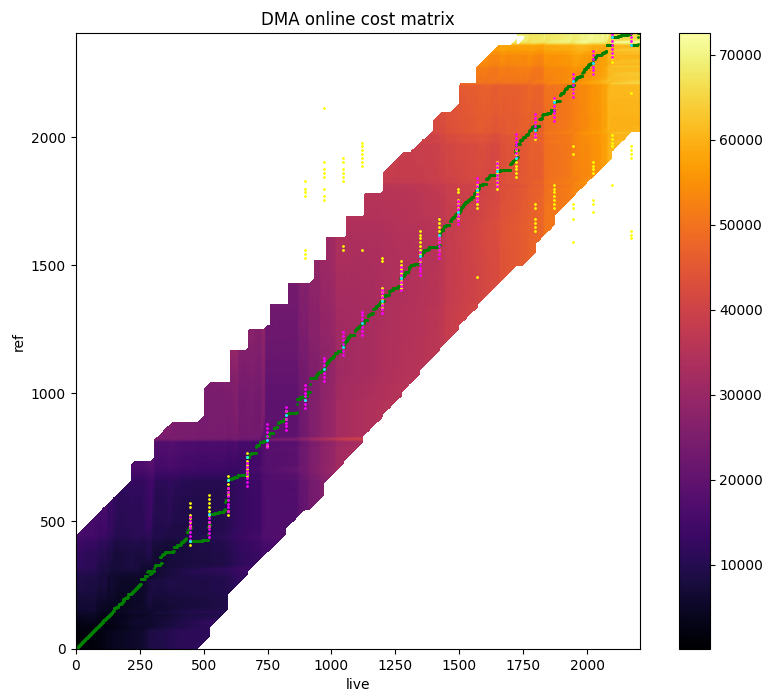
\includegraphics[scale=0.36]{ch4/fig-mss-140bpm-tracking-system-output.png}}
    ~
    \subcaptionbox
    {
    \label{fig:mss-140bpm-comparision-output}}
    {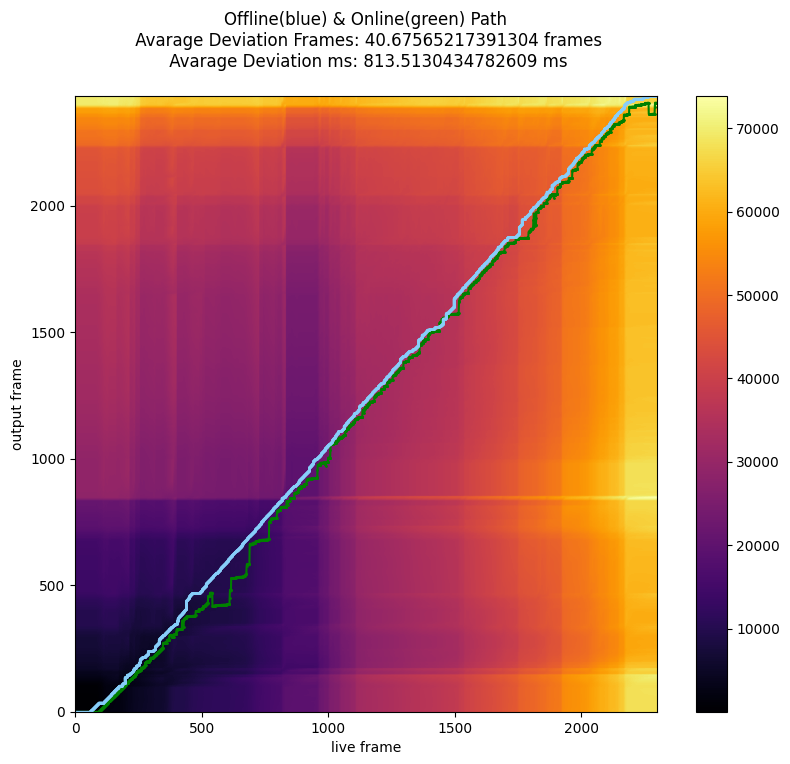
\includegraphics[scale=0.36]{ch4/fig-mss-140bpm-offline-and-online-output.png}}
    \caption{140bpm 平均延遲:40.68 幀}
    \label{fig:fig-ch4-mss-140bpm-tracking-results}
\end{figure}

\cref{fig:fig-ch4-mss-free-tracking-results}為自由速度下的追蹤結果,
由\cref{fig:mss-free-tracking-output}的xy軸可以看出現場音訊比參考音訊的速度稍慢一些,
在live frame約1500之後,可以看到追蹤的路徑並不穩定,我認為可能是這段的旋律是重複的,
因此可能在粗略估計的位置上無法精準的計算目前粗估位置,但最後還是有走回正軌。
\cref{fig:mss-free-comparision-output}顯示了追蹤結果與離線計算結果的延遲為28.43幀,
約為569ms左右。

\begin{figure}[H]
    %\captionsetup[subfigure]{labelformat=empty} % 完全隱藏圖號
    \centering
    \subcaptionbox
    {
    \label{fig:mss-free-tracking-output}}
    {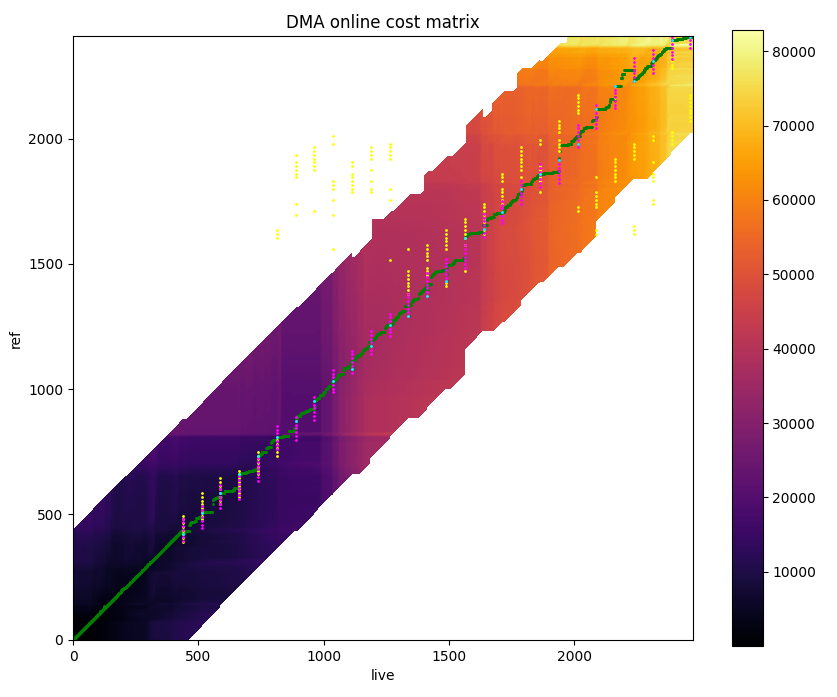
\includegraphics[scale=0.36]{ch4/fig-mss-free-tracking-system-output.png}}
    ~
    \subcaptionbox
    {
    \label{fig:mss-free-comparision-output}}
    {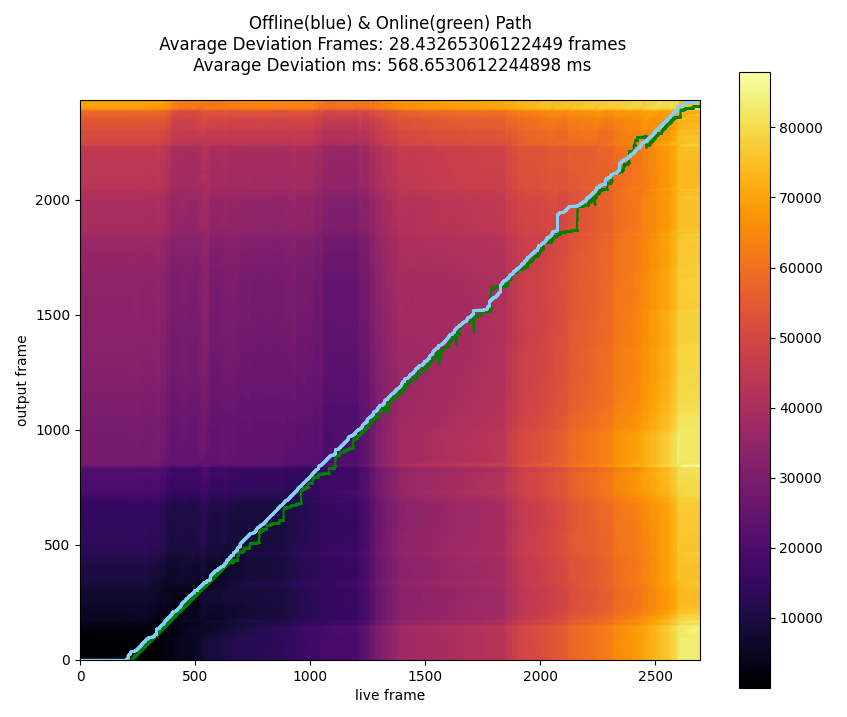
\includegraphics[scale=0.36]{ch4/fig-mss-free-offline-and-online-output.png}}
    \caption{自由速度 平均延遲:28.43 幀}
    \label{fig:fig-ch4-mss-free-tracking-results}
\end{figure}

由於參考音訊與現場音訊的特徵不一致,導致ODTW在計算對齊點時穩定性較為不足,
RPE估計出的位置也因為兩個音訊的特徵不夠相近,使粗略估計的位置偏差較嚴重,
因此追蹤結果圖大多數看起來比\ref{ch4-subst-midi-tracking-results}節的結果要差。
但可以看到在比較離線對齊路徑與線上對齊路徑的結果圖,大致上的路徑都與離線對齊路徑重合,
因此我們可以知道這兩個音訊在線上的最佳對齊路徑已經非常接近離線對齊路徑,
達到了即使使用不同特徵追蹤也能維持離線最佳對齊的效果。
另外可以看到比較圖中從第0幀到兩段路徑開始對齊的時間點是一致的,
代表我們的Music detector在判斷演奏者的演奏時間是精準的。
此外,我認為平均延遲都高達500ms以上可能是因為DTW在計算對齊路徑時,i與j都有遵守連續性的限制,
因此不會出現一次跳2格以上的路徑,且i是可以重複的;
但我們在計算ODTW時,在j方向是有可能出現一次跳2格以上的路徑,然而i為嚴格遞增,
因此造成兩個路徑在計算時,因為固定了i的位置,在$(t_j-t_i)$的差距可能會更大,
但實際聽起來並沒有延遲500ms那麼多。

我們也測試了使用同一人演奏的參考特徵來追蹤現場演奏的效果,
首先我們先錄製了與伴奏音訊完整對齊的音訊作為參考音訊,接著現場演奏我們一樣採自由速度,
聆聽伴奏音訊來演奏,結果如\cref{fig:fig-ch4-free-ours-ref-tracking-results}所示,
可以看到線上對齊路徑與離線對齊路徑重合,代表系統輸出的路徑是最佳對齊位置,
在平均延遲上也比\cref{fig:fig-ch4-mss-free-tracking-results}要來的好。

\begin{figure}[H]
    %\captionsetup[subfigure]{labelformat=empty} % 完全隱藏圖號
    \centering
    \subcaptionbox
    {
    \label{fig:free-ours-ref-tracking-output}}
    {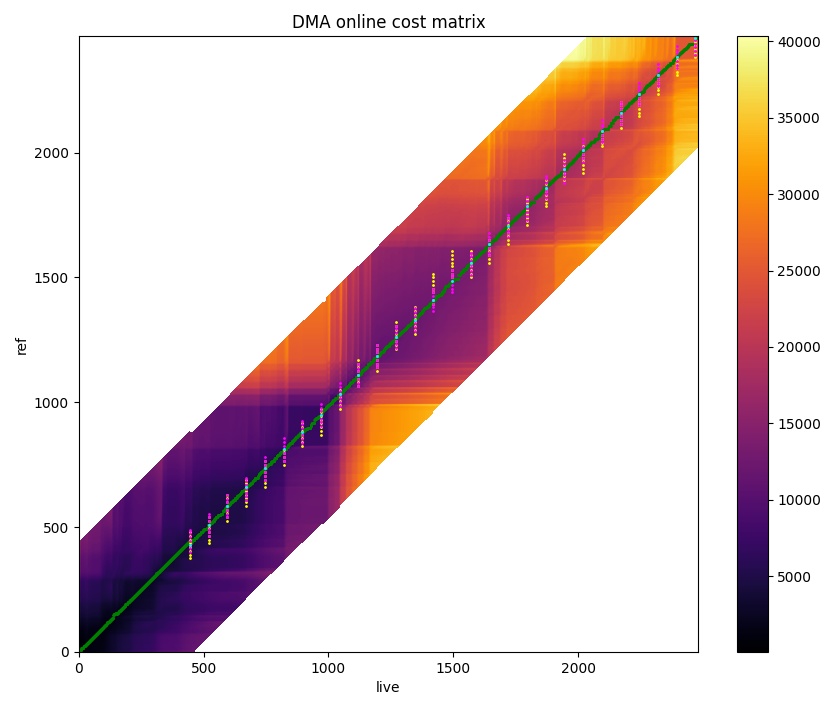
\includegraphics[scale=0.36]{ch4/fig-free-ours-ref-tracking-system-output.png}}
    ~
    \subcaptionbox
    {
    \label{fig:free-ours-ref-comparision-output}}
    {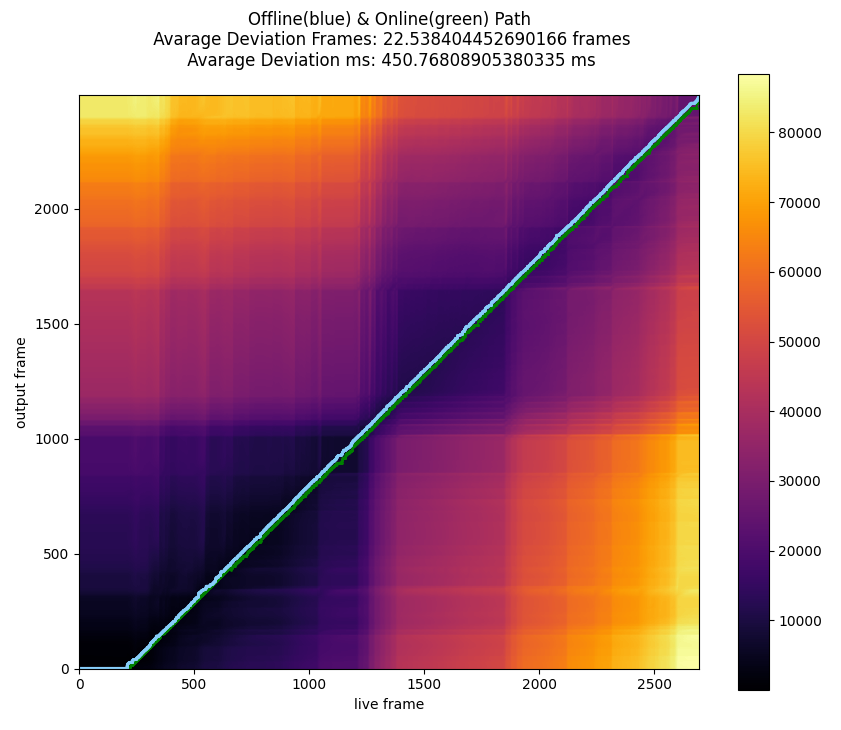
\includegraphics[scale=0.36]{ch4/fig-free-ours-ref-offline-and-online-output.png}}
    \caption{自由速度(參考音訊為同一人所演奏) 平均延遲:22.54 幀}
    \label{fig:fig-ch4-free-ours-ref-tracking-results}
\end{figure}

% cost matrix對齊圖
% dtw vs ODTW對齊圖

% \subsection{不同系統參數設定下的追蹤結果}
% 需測試

\pagebreak

\end{document}